\documentclass[10pt, a4paper]{report}
\usepackage[backend=bibtex,style=numeric]{biblatex}
\usepackage[justification=centering]{caption}
\usepackage[pdfpagelabels,bookmarks,hyperindex,hyperfigures, hidelinks]{hyperref}
\usepackage[toc, page]{appendix}
\usepackage[utf8]{inputenc}
\usepackage[version=4]{mhchem}
\usepackage{alltt}
\usepackage{amsmath}
\usepackage{booktabs}
\usepackage{circuitikz}
\usepackage{comment}
\usepackage{csquotes}
\usepackage{epstopdf}
\usepackage{fancyhdr}
\usepackage{gensymb}
\usepackage{hyphsubst}
\usepackage{lastpage}
\usepackage{multirow}
\usepackage{parskip}
\usepackage{pdfpages}
\usepackage{placeins}
\usepackage{subcaption}
\usepackage{tabularx}
\usepackage{textcomp}
\usepackage{tikz}
\usepackage{titlesec}
\usepackage{upgreek}
\usepackage{wrapfig}
\usepackage{xfrac}
\usepackage{pdfpages}
\usepackage{multicol}

\usetikzlibrary{arrows, arrows.meta, decorations.markings, positioning}
\addbibresource{autobench_doc.bib}

% if definition for section compilling control
\newif\ifdebug
%\debugtrue
\debugfalse

\setlength{\parskip}{0.6em}

% Set the indentation length 
\setlength{\parindent}{0em}


% Glossary entries
\usepackage[acronym, nomain]{glossaries}
\makenoidxglossaries

\newacronym{CPU}{CPU}{Central Processing Unit}
\newacronym{DCLS}{DCLS}{Dual core Lockstep}
\newacronym{DD}{DD}{Displacement Damage}
\newacronym{DLD}{DLD}{Deep Level detector}
\newacronym{ECC}{ECC}{Error Correction Codes}
\newacronym{FI}{FI}{Functional Interrupts}
\newacronym{FTM}{FTM}{Fault Tolerance Monitor}
\newacronym{MCU}{MCU}{Microcontroller Unit}
\newacronym{NMR}{NMR}{N-Modular Redundancy}
\newacronym{PC}{PC}{Program Counter}
\newacronym{QOS}{QOS}{Quality of Service}
\newacronym{SDC}{SDC}{Silent Data Corruption}
\newacronym{SEEs}{SEEs}{Single-Event Effects}
\newacronym{SEFIs}{SEFIs}{Single-Event Functional Interrupts}
\newacronym{SET}{SET}{Single-Event Transient}
\newacronym{SEU}{SEU}{Single-Even Upset}
\newacronym{TID}{TID}{Total Ionizing Dose}
\newacronym{TMR}{TMR}{Triple Modular Redundancy}
\newacronym{DWC}{DWC}{Duplication with Comparisson}
\newacronym{SIHFT}{SIHFT}{Software-implemented hardware fault tolerance}
\newacronym{ABFT}{ABFT}{Algorithm-Based Fault Tolerance}
\newacronym{HETA}{HETA}{Hybrid Error-Detection Technique Using Assertions}
\newacronym{SSETA}{S-SETA}{Selective Software-Only Error-Detection Technique
Using Assertions}
\newacronym{SWIFT}{SWIFT}{Software Implemented Fault Tolerance}
\newacronym{SWIFTR}{SWIFT-R}{Software Implemented Fault Tolerance with Recovery}
\newacronym{SSWIFTR}{S-SWIFT-R}{Selective Software Implemented Fault Tolerance 
with Recovery}
\newacronym{IP}{IP}{Intellectual Property}
\newacronym{ISA}{ISA}{Instruction Set Architecture}


\tikzstyle{vecArrow} = [thick, decoration={markings,mark=at position
	1 with {\arrow[semithick]{open triangle 60}}},
double distance=1.4pt, shorten >= 5.5pt,
preaction = {decorate},
postaction = {draw,line width=1.4pt, white,shorten >= 4.5pt}]
\tikzstyle{innerWhite} = [semithick, white,line width=1.4pt, shorten >= 4.5pt]
\graphicspath{{assets/}} 
\newcommand\reaction[1]{\begin{equation}\ce{#1}\end{equation}} 

\titleclass{\subsubsubsection}{straight}[\subsection]

\newcounter{subsubsubsection}[subsubsection]
\renewcommand\thesubsubsubsection{\thesubsubsection.\arabic{subsubsubsection}}
\renewcommand\theparagraph{\thesubsubsubsection.\arabic{paragraph}} % optional; useful if paragraphs are to be numbered

\titleformat{\subsubsubsection}
  {\normalfont\normalsize\bfseries}{\thesubsubsubsection}{1em}{}
\titlespacing*{\subsubsubsection}
{0pt}{3.25ex plus 1ex minus .2ex}{1.5ex plus .2ex}

\makeatletter
\renewcommand\paragraph{\@startsection{paragraph}{5}{\z@}%
  {3.25ex \@plus1ex \@minus.2ex}%
  {-1em}%
  {\normalfont\normalsize\bfseries}}
\renewcommand\subparagraph{\@startsection{subparagraph}{6}{\parindent}%
  {3.25ex \@plus1ex \@minus .2ex}%
  {-1em}%
  {\normalfont\normalsize\bfseries}}
\def\toclevel@subsubsubsection{4}
\def\toclevel@paragraph{5}
\def\toclevel@paragraph{6}
\def\l@subsubsubsection{\@dottedtocline{4}{7em}{4em}}
\def\l@paragraph{\@dottedtocline{5}{10em}{5em}}
\def\l@subparagraph{\@dottedtocline{6}{14em}{6em}}
\makeatother

\setcounter{secnumdepth}{4}
\setcounter{tocdepth}{4}

\setcounter{MaxMatrixCols}{20}

\setlength{\headheight}{52pt}
\pagestyle{fancy}
\fancyheadoffset{0.5cm}
\fancyhead{}
\fancyhead[L]{
\includegraphics[scale=0.3]{ida.png}}
\fancyhead[C]{Technische Universität Braunschweig\\
Institut für Datentechnik und Kommunikationsnetzte}
\fancyhead[R]{
\includegraphics[scale=0.2]{tub.png}}

\renewcommand{\figurename}{Fig.}

\renewcommand\footrule{\begin{minipage}{0.95\textwidth}
    \hrule width \hsize   
\end{minipage}\par}

\setlength{\footskip}{30pt}
\fancyfoot[L]{\textit{M. Moya}}
\fancyfoot[C]{}
\fancyfoot[R]{\textit{Page \thepage{} de \pageref{LastPage}}}

\DeclareGraphicsExtensions{.bmp, .png, .jpg}

\topmargin = -1.5cm
\leftmargin = -1cm
\oddsidemargin = 0cm
\textheight = 24cm
\textwidth = 17cm

% renew itemize symbol level II
\renewcommand{\labelitemii}{$>$}

\begin{document}

\ifdebug
DebugOn
\newpage
\else
\begin{titlepage}
    \begin{center}
	\begin{minipage}{.45\textwidth}
	    \flushleft
	    
\includegraphics[scale=0.5]{ida.png}
	\end{minipage}%
	\begin{minipage}{.45\textwidth}
	    \flushright
	    
\includegraphics[scale=0.41]{tub.png}
	\end{minipage}

	\vspace{15mm}

	\large{ \textbf{Technische Universität Braunschweig}} \\[5mm]
	\textbf{Institut für Datentechnik und Kommunikationsnetze} \\[50mm]
	\Large{\textbf{Error Handling within a Dual Core Lockstep RISC-V Processor
    Architecture}} \\[15mm]

    \end{center}

    {\large\textbf{Author(s):}}
    \begin{itemize}
        \item [] Martin Moya - \texttt{m.moya@tu-braunschweig.de}
    \end{itemize}
    \vspace{10pt}
    {\large\textbf{Supervisor(s):}}

    \begin{itemize}
        \item [] Alexander Dörflinger - \texttt{adoerflinger@ida.ing.tu-bs.de}
    \end{itemize}
    \vspace{10pt}
    {\large\textbf{Examiner(s):}}
    \begin{itemize}
        \item [] Prof. Dr.-Ing. Rolf ernst - \texttt{ernst@ida.ing.tu-bs.de}
        \item [] Prof. Dr.-Ing. Harald Michalik - \texttt{michalik@ida.ing.tu-bs.de}
    \end{itemize}
    \vspace{10pt}
\end{titlepage}

\newpage

\begin{abstract}
    \thispagestyle{fancy}
    Microcontrollers (\acrshort{MCU}) are widely used in critical applications 
    due to low-energy consumption and high-performance computing power. Despite 
    these advantages, \acrshort{MCU}s are sensitive to radiation like any other
    electronic device, leading to transient and interminent faults causing
    cathastrophic situations.

    Critical applications have to function in a proper manner and deliver high
    level of \acrlong{QOS} (\acrshort{QOS}), on the other hand, these kind of
    applications have also strict time and cost constrains, which means that
    they do not only have to meet high \acrshort{QOS} standards, they also have
    to satisfy with a handfull of constraints. In order to adress these issues, 
    this work analyzes and proposes the development of a software solution for 
    error handling within a Dual Core Lockstep (\acrshort{DCLS}) RISC-V 
    Processor Architecture. The solution provides a framework to implement 
    different error handling techniques given specific scenarios in order to 
    satisfy both requirements.
\end{abstract}

\newpage
% Print table of contents
\begin{tableofcontents}
    \thispagestyle{fancy}
\end{tableofcontents}

\newpage

\chapter{Introduction}

\thispagestyle{fancy}
A system is considered \emph{Safety-critical} when a failure in such could
result in loss of life, significant property damage, or damage to the
environment. Aircrafts, cars, weapons systems, medical devices and nuclear 
plants are considered traditional examples of safety-critical systems. Most of 
these applications, if not all, rely on embedded systems that are expected to be 
fault tolerant. A system fault tolerant, according to the authors in 
\ref{nasa_fault_tolerance}, is a system that is able to continue operating 
without interruption when one or more of its components fail, they aim 
to provide the ability to deliver a service that can be trusted, while fault 
removal and fault forecasting aim to reach confidence in that ability by 
justifying that the functional and the dependability and security specifications 
are adequate and that such system is likely to meet them.

The objective of creating a fault-tolerant system is to prevent disruptions
arising from a single point of failure, ensuring the high availability and
business continuity of mission-critical applications or systems. As of now there
are three known kinds of high-level faults in embedded systems, such faults can 
be permanent, intermittent or transient. Permanent faults cause long-term 
malfunctioning of components, while transient and intermittent faults appear for 
a short time. The effects of these faults, independently of their nature, can be 
devastating. They may corrupt data or lead to logic miscalculations, which can 
result in a fatal failure or dramatic \acrshort{QOS} deterioration if not 
handled properly. 

Transient and intermittent faults can be addressed in \emph{hardware} with
hardening techniques, in the \emph{software} domain, simulating the
\emph{hardware} solutions within the firmware itself and a hybrid solution
between both domains. Safety-critical applications have to be implemented in 
such a way that they satisfy strict timing requirements and tolerate faults 
without exceeding a given amount of resources or an specific time requirement. 
Moreover, not only timeliness, reliability and cost-related requirements have to 
be considered but also other issues such as debugability and testability must be
taken into account.

\section{Motivations}

In this section, it is described the motivation of the analysis and 
implementation of software error handling techniques for fault tolerant systems 
during the design of safety-critical applications based on a RISC-V 
\acrshort{DCLS} architecture, describing the current issues with \acrshort{MCU} 
and soft errors as well as possible solutions to this problem. Finally, it is 
also introduced the starting point of the proyect and a short overview of the 
work's structure.

\subsection{Soft errors and their effects in processors}

A soft error is a \emph{glitch} in a semiconductor device. These glitches are
random and usually cathastrophic in safety-critical application. The main source
of soft error come from \emph{ionizing radiation}. Ionizing radiation are
high-energy particles (e.g. alpha particles, heavy ions, neutrons) or
electromagnetic waves (e.g. X-rays, gamma rays) striking the semiconductor
substrate provoking faults which lead to soft errors in such devices under
radiation. While these errors have a transient behaviour that does not
permamently harm digital/analogue circuits, they have a significant impact on
system reliability; thus, as mentioned before, leading to catasthrope in a
safety-critical application. Ionizing radiation can potentially harm electronics
in three major ways:

\begin{enumerate}

    \item \textbf{\acrfull{TID}}: which relates to an electronic device's
        accumulated, irreversible damage (i.e. hard error) that results in the
        degradation of the device over the time. It happens when charge carriers
        are inserted, as radiation strikes, into the isulators of the device,
        where they are trapped and thereby change the electrical
        characteristics.
    \item \textbf{\acrfull{SEEs}}: These faults are most frequently temporary
        (i.e. soft error) and do not cause permanent harm like \acrshort{TID};
        however, they can provoke undesired changes in behaviour. Excess charge
        carriers, produced as silicon atoms get ionized under radiaton, are
        responsible for these transient effects. If a large amount of these
        charges accumulates in a particular region, an event called 
        \acrfull{SET} might arise where logical values of lines in that region
        are briefly disrupted untill the dissipation of the excess charges.
        Nevertheless, if a storage unit latches the new value of a line, a
        longer lasting effect on the system output, i.e. \acrfull{SEU}, will
        occur which can generally be resolved by restoring all values through a
        system reset. However, \acrfull{SEFIs}, a type of \acrshort{SEU}, cannot
        be dealt with a simple reset.
    \item \textbf{\acrfull{DD}}: This kind of iraddiation effect occurs when a
        high-speed particle hits and displaces silicon atoms from their
        locations. These movements cause defects in the silicon substrate; thus,
        the electrical features of the device are altered.
\end{enumerate}

These three kinds of irradiation impact differently in the \acrshort{MCU}s
behavior, as \acrshort{TID} and \acrshort{DD} effects do irreversible permanent 
damage to the device, this work focus mostly on \acrshort{SEEs} irradiation
effects.

\acrshort{SEU}s can readily affect the data-flow and control-flow of a
process. Upsets in values stored in memory elements can lead to data-flow errors 
cause by the execution of an incorrect operation or data manipulation. The
execution of an incorrect operation occurs when a bit-flip corrupts the program
code, leading to an incorrect instruction. On the other hand, if the bit-flip
affects data used as an input by an operation, outputs of that operation would
most probably be incorrect. In both types of data-flow errors, the final outputs
of the application would be inaccurate, which is classified as \acrshort{SDC}.

When a \acrshort{SEU} affects the control-flow, the processor may execute the
program incorrectly, thus causing either an application crash or a processor
hang, which is classified as \acrshort{FI}s. Upsets in the control-flow may lead
to branch errors, such as erroneous creation or deletion of a branch and
incorrect branch decision. The erroneous creation is due to a bit-flip that sets
a non-branch instruction into a branch, which leads the program flow to an
incorrect address, whereas the erroneous deletion occurs when the branch
instruction is transformed into another instruction; thus, a due branch may not
be taken. A bit-flip in a conditional branch may also result in an incorrect
decision regarding holding the target address of a branch instruction, thus
assigning an incorrect address to the program execution. Moreover, if the
\acrfull{PC} is affected by a soft error, the next instruction to be executed
changes, leading the program flow to an incorrect address.

These situations, in the context of a \emph{Safety-critical} system, makes
necessary the development of \emph{fault-tolerant} embedded systems. As
mentioned earlier, there are several solutions in three specific domains,
\emph{hardware}, \emph{software} and \emph{hybrid} with a broad spectrum of
techniques.

\subsection{Fault-tolerance techniques}

The hardware-based techniques, rely solely on spatial redundancy, providing two
or more instances of a hardware component, such as processors, memories, buses
or power supplies, for protection agains soft errors. This class of techniques
include \acrfull{TMR}, \acrfull{DWC} and hardware monitors which incorporate
watchdog or checker modules to monitor the system and detect errors. These
techniques can protect the system from rrors in the computations outputs. i.e.
\acrshort{SDC}s.

On the other hand, Software

\begin{comment}
A \acrshort{DCLS} RISC-V based architecture has been already proposed and
designed in \ref{ida_fault_tolerance_framework}, according to its authors it
includes different hardware hardening techniques such as 
\acrlong{NMR} Crossbar (\acrshort{NMR}) and a \acrlong{DLD} (\acrshort{DLD}) to
protect logic and registers,
\acrlong{ECC} (\acrshort{ECC}) blocks in different memory arrays (such as cache
and other kind of memories) and a \acrlong{FTM} (\acrshort{FTM}) as can be seen 
in Figure \ref{ida_fault_tolerance_arch}.

\begin{figure}[h!]
    \begin{center}
        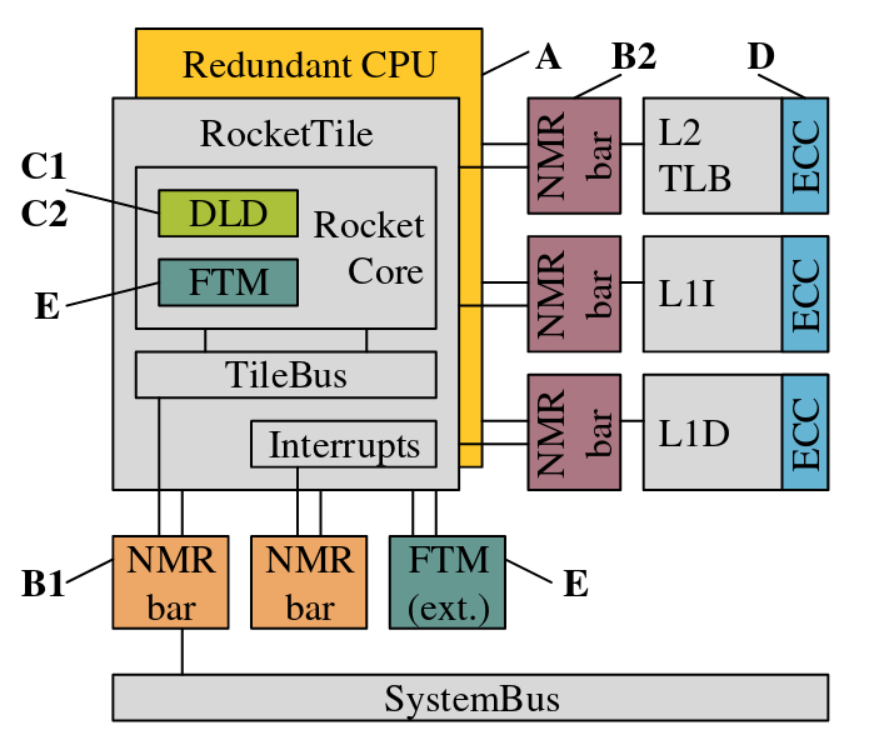
\includegraphics[width=0.7\textwidth]{idafaulttolerancearch.png}
        \caption{Block Diagram from the Fault Tolerant RISC-V architecture
        designed in \ref{ida_fault_tolerance_framework}. The \acrshort{DCLS} can
    be clearly seen by the redundant \acrlong{CPU} (\acrshort{CPU}).}
        \label{ida_fault_tolerance_arch}
    \end{center}
\end{figure}

Furthermore, this framework allows developers and researchers to easily modify 
it and implement different hardware hardening techniques. Although all its benefits
and great error detection and mitigation results, this framework lacks of
software error handling and recovery techniques such as, for example,
checkpointing for rollback or roll-forward recovery, global reset 

\end{comment}

\newpage

% Print table of acronyms
\addcontentsline{toc}{section}{Tabla de Abreviaturas}
\glsaddall
\printnoidxglossary[type=\acronymtype,title={Abreviaturas}]

\end{document}
